% !TEX root = main.tex

%%%-------------------------------------------
\section*{Листочек 7: рекуррентные сети} 

\addcontentsline{toc}{section}{Листочек 7: рекуррентные сети}

\epigraph{А сегодня в завтрашний день, не все могут смотреть. Вернее смотреть могут не только лишь все, не каждый может это делать.}{\textit{Рекуррентная сеть глубины один}}


\begin{problem}{(Туда и обратно)}
Маша хочет сделать шаг обратного распространения ошибки через рекуррентную ячейку для последовательности $y_0 = 0, y_1=1, y_2 = -1, y_3 =2$. Скрытое состояние инициализировано как $h_0 = 0$. Все веса инициализированы как $0.5$. Во всех уравнениях, описывающих ячейку нет констант. В качестве функций активаций Маша использует $ReLU$. В качестве функции потерь Маша использует $MSE$. 

\begin{center}
	\definecolor{zzttqq}{rgb}{0.6,0.2,0.}
	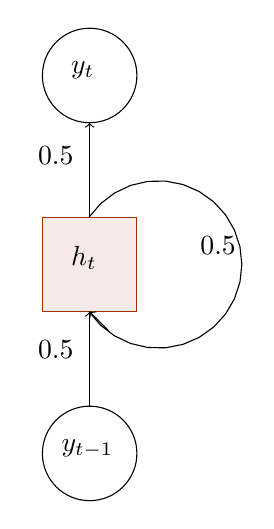
\begin{tikzpicture}[scale=0.6]
			\fill[line width=2.pt,color=zzttqq,fill=zzttqq,fill opacity=0.10000000149011612] (2.,8.) -- (2.,6.) -- (4.,6.) -- (4.,8.) -- cycle;
			\draw  (3.,3.) circle (1.cm);
			\draw [color=zzttqq] (2.,8.)-- (2.,6.);
			\draw [color=zzttqq] (2.,6.)-- (4.,6.);
			\draw [color=zzttqq] (4.,6.)-- (4.,8.);
			\draw [color=zzttqq] (4.,8.)-- (2.,8.);
			\draw (3,11) circle (1.cm);
			\draw [->] (3,4) -- (3,6); 
			\draw [->] (3,8) -- (3,10);
			\draw [shift={(4.45,7.)}]  plot[domain=-2.541806576912956:2.541806576912956,variable=\t]({1.*1.7715861960215864*cos(\t r)+0.*1.7715861960215864*sin(\t r)},{0.*1.7715861960215864*cos(\t r)+1.*1.7715861960215864*sin(\t r)});
			\draw [->] (3.4,5.6) -- (3,6.);
			\draw (2.2,3.5) node[anchor=north west] {$y_{t-1}$};
			\draw (2.4,11.5) node[anchor=north west] {$y_t$};
			\draw (6.3,7.8) node[anchor=north east] {$0.5$};
			\draw (2.4,7.6) node[anchor=north west] {$h_t$};
			\draw (1.7,9.7) node[anchor=north west] {$0.5$};
			\draw (1.7,5.6) node[anchor=north west] {$0.5$};
	\end{tikzpicture}
\end{center}

    \begin{enumerate} 
    \item Сделайте прямой шаг через ячейку. Для каждого элемента последовательности постройте прогноз. Посчитайте значение ошибки. 
    \item Сделайте обратный шаг распространения ошибки. Посчитайте для каждого из весов градиенты и обновите значения весов.
    \end{enumerate} 
\end{problem}


\begin{problem}{(Число параметров)}
У Маши есть очень длинный временной ряд. Она хочет обучить несколько нейросетей предсказывать его дальнейшее значение. В своих моделях Маша нигде не использует константы. 

\begin{enumerate} 
    \item Маша выделяет окно длины $100$. Оно движется по последовательности. Для каждого окна Маша предсказывает следующее значение в ряду. В сетку подаются наблюдения с $1-$го по $100-$е. Прогнозируется $101-$ое наблюдение. Затем на вход подаются наблюдения со $2-$го по $100-$е. Прогнозируется $102-$ое наблюдение. И так далее до конца последовательности.
    
    На первом слое используется $20$ нейронов. На втором слое используется один нейрон. Сколько параметров нужно оценить? 
    % 100*20 + 20*1 = 2020 
    
    \item Маша использует одну простую RNN-ячейку. Сколько параметров ей необходимо оценить? 
    % 3
    
    \item Маша хочет предсказывать значение $y_t$ по трём последовательностям $y_{t-1},$ $y_{t-2}$ и $y_{t-3}.$ На первом слое сети Маша использует два рекуррентных нейрона. На втором слое она использует один рекуррентный нейрон. Матрица какого размера идёт на вход в первый слой? Матрица какого размера передаётся во второй слой? Какое число параметров необходимо оценить Маше? 
    
    \item Мы находимся в условиях прошлого пункта, но используетм LSTM-ячейки с забыванием. Сколько параметров надо оценить? 
    
    \item Мы находимся в условиях прошлого пугкта, но используем GRU-ячейки. Сколько параметров надо оценить?
\end{enumerate} 
\end{problem}


\begin{problem}{(Из картинки в формулу)}
    У Маши есть два рекуррентных нейрона. Помогите ей изобразить их в виде вычислительных графов.
    
    \begin{minipage}{0.45\linewidth} 
    \textbf{Однонаправленный:}
    	\begin{equation*} 
        	\begin{aligned}
        	h_t =& f_h(b_h + W \cdot h_{t-1} + V \cdot x_t)\\
        	y_t =& f_y(b_y + U \cdot h_t)
        	\end{aligned}
    	\end{equation*} 
    \end{minipage}
    \hfill
    \begin{minipage}{0.45\linewidth} 
    \textbf{Двунаправленный:}
    	\begin{equation*} 
        	\begin{aligned}
        	h_t =& f_h(b_h + W \cdot h_{t-1} + V \cdot x_t)\\
        	s_t =& f_s(b_s + W' \cdot s_{t+1} + V' \cdot x_t)\\
        	o_t =& b_y + U \cdot h_t + U' \cdot s_t \\
        	y_t =& f_y(o_t)
        	\end{aligned}
    	\end{equation*} 
    \end{minipage}
    
\end{problem}

\begin{problem}{(Замочные скважины)}
В 2000 году Шмидхубер и Герс предложили модификацию LSTM с замочными скважинами. Она описывается следующей системой из уравнений 

\begin{equation*} 
	\begin{aligned}
	c'_t &= \phi_c(W_c x_t + V_c h_{t-1} + b_c) \\
	i_t &= \phi_i(W_i x_t + V_i h_{t-1} + U_i c_{t-1} + b_i) \\
	f_t &= \phi_f(W_f x_t + V_f h_{t-1} + U_f c_{t-1} + b_f) \\
    o_t &= \phi_o(W_o x_t + V_o h_{t-1} + U_o c_{t-1} + b_o) \\
    c_t &= f_t \odot c_{t-1} + i_t \odot c'_t \\
    h_t &= o_t \odot \phi_h(c_t) \\
	\end{aligned}
\end{equation*} 

Изобразите эту ячейку в виде вычислительного графа. Объясните, чем именно она отличается от базовой модификации LSTM. Какой в этом смысл?
\end{problem}


\begin{problem}{(Лишние части)}
Выпишите уравнения, описывающие LSTM-ячейку с забыванием и GRU-ячейку. Какие последовательности и веса нужно занулить, чтобы эти ячейки превратились в простую RNN-ячейку? 
\end{problem}


\newpage



		\begin{center}
		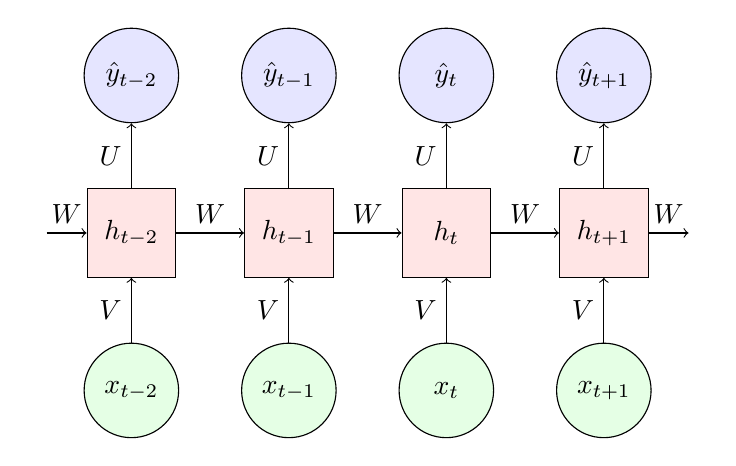
\begin{tikzpicture}
			\tikzstyle{place}=[circle, draw=black, minimum size = 12mm]
			\tikzstyle{placeh}=[minimum height=32pt,minimum width=32pt, inner sep=2pt, draw=black]
			
			\node at (-1.2,0) (here) {};
			
			\draw node at (0, 2) [place, fill=blue, opacity=0.1] (y) {$\hat y_{t-2}$};
			\draw node at (0, 2) [place] {$\hat y_{t-2}$};  % мои костыли максимально всратые
			\draw node at (0, 0) [placeh, fill=red, opacity=0.1] (h) {$h_{t-2}$};
			\draw node at (0, 0) [placeh] {$h_{t-2}$};
			\draw node at (0, -2) [place, fill=green, opacity=0.1] (x) {$x_{t-2}$};
			\draw node at (0, -2) [place] {$x_{t-2}$};
				
			\draw [->]  (here) to node[above]{$W$} (h);
			\draw [->]  (x) to node[left]{$V$} (h);
			\draw [->]  (h) to node[left]{$U$} (y);
			
			\draw node at (2, 2) [place, fill=blue, opacity=0.1] (y1) {$\hat y_{t-1}$};
			\draw node at (2, 2) [place] {$\hat y_{t-1}$};  % мои костыли максимально всратые
			\draw node at (2, 0) [placeh, fill=red, opacity=0.1] (h1) {$h_{t-1}$};
			\draw node at (2, 0) [placeh] {$h_{t-1}$};
			\draw node at (2, -2) [place, fill=green, opacity=0.1] (x1) {$x_{t-1}$};
			\draw node at (2, -2) [place] {$x_{t-1}$};
			
			\draw [->]  (h) to node[above]{$W$} (h1);
			\draw [->]  (x1) to node[left]{$V$} (h1);
			\draw [->]  (h1) to node[left]{$U$} (y1);
			
			\draw node at (4, 2) [place, fill=blue, opacity=0.1] (y2) {$\hat y_{t}$};
			\draw node at (4, 2) [place] {$\hat y_{t}$};  % мои костыли максимально всратые
			\draw node at (4, 0) [placeh, fill=red, opacity=0.1] (h2) {$h_{t}$};
			\draw node at (4, 0) [placeh] {$h_{t}$};
			\draw node at (4, -2) [place, fill=green, opacity=0.1] (x2) {$x_{t}$};
			\draw node at (4, -2) [place] {$x_{t}$};
			
			\draw [->]  (h1) to node[above]{$W$} (h2);
			\draw [->]  (x2) to node[left]{$V$} (h2);
			\draw [->]  (h2) to node[left]{$U$} (y2);
			
			
			\draw node at (6, 2) [place, fill=blue, opacity=0.1] (y3) {$\hat y_{t+1}$};
			\draw node at (6, 2) [place] {$\hat y_{t+1}$};  % мои костыли максимально всратые
			\draw node at (6, 0) [placeh, fill=red, opacity=0.1] (h3) {$h_{t+1}$};
			\draw node at (6, 0) [placeh] {$h_{t+1}$};
			\draw node at (6, -2) [place, fill=green, opacity=0.1] (x3) {$x_{t+1}$};
			\draw node at (6, -2) [place] {$x_{t+1}$};
			
			\draw [->]  (h2) to node[above]{$W$} (h3);
			\draw [->]  (x3) to node[left]{$V$} (h3);
			\draw [->]  (h3) to node[left]{$U$} (y3);
			
			\node at (7.2,0) (end) {};
			\draw [->]  (h3) to node[above]{$W$} (end);
		\end{tikzpicture}
	\end{center}
	
	
% https://tex.stackexchange.com/questions/432312/how-do-i-draw-an-lstm-cell-in-tikz/432344


